\chapter{Kryptographische Sicherheitsbegriffe}
\section{Sicherheitsparameter und effiziente Angreifer}\label{sec:secparam}
Zu einer Funktion, für die sicherheitsrelevante Eigenschaften gefordert werden, wird in der Kryptographie oft ein \emph{Sicherheitsparameter} $k$ definiert. Informell gesagt, legt $k$ das Sicherheitsniveau der Funktion fest. Beispielsweise parametrisiert er den Schlüsselraum eines Verschlüsselungsverfahrens, was es schwieriger macht, den korrekten Schlüssel zu raten oder per Brute-Force zu berechnen.
\begin{beispiel}
	Wir betrachten ein symmetrisches Verschlüsselungsverfahren für das als Schlüsselraum $\{0,1\}^k$ verwendet wird und die Schlüssel gleichverteilt zufällig gezogen werden. Die Schlüssel sind also Bitstrings der Länge $k$ und es existieren $2^k$ mögliche Schlüssel. Somit muss ein Angreifer im Worst-Case bei der Brute-Force Methode $2^k$ Schlüssel durchprobieren oder kann den korrekten Schlüssel durch (einmaliges) Raten mit Wahrscheinlichkeit $1/2^k$ bestimmen. 
	\begin{description}
		\item[Fall $k=128$:] Es existieren $2^{128} > 3.4 \cdot  10^{38}$ mögliche Schlüssel. 
		\item[Fall $k=512$:] Es existieren $2^{512} > 1.3 \cdot 10^{154}$ mögliche Schlüssel. Zum Größenvergleich: 
		Die Anzahl an Atomen im sichtbaren Universum wird häufig auf $10^{80}$ geschätzt.  
	\end{description}
	
\end{beispiel}

Zur Analyse der Sicherheitseigenschaften eines kryptographischen Verfahrens betrachtet man hauptsächlich Angreifer, die \emph{effizient}, das heißt in ihrer Rechenzeit geeignet eingeschränkt sind. In der Komplexitätstheorie und auch in der Kryptographie wird ein effizienter Algorithmus mit einer polynomial-beschränkten Laufzeit in der Eingabegröße gleichgesetzt. 
In anderen Worten ist ein Algorithmus bei Eingabe eines Bit-Strings der Länge $n$ genau dann effizient, wenn es ein $c \in \mathbbm{N}$ gibt, so dass seine Laufzeit im schlechtesten Fall in $O(n^c)$ liegt. Wie betrachten in der Kryptographie also asymptotische Sicherheit, ähnlich wie die asymptotische Laufzeitbetrachtung in der Algorithmik.

Um präzise über die Laufzeit im Bezug auf den Sicherheitsparameter argumentieren zu können, erhalten Algorithmen und Angreifer den Bit-String $1^k$ als Eingabe (hiermit ist der Bitstring bestehende aus $k$ Einsen gemeint). Ihre Rechenzeit ist damit also durch den Sicherheitsparameter $k$ begrenzt.\footnote{Deshalb wird auch $1^k$ statt $k$ übergeben, da $k$ mithilfe von nur $\log(k)$ Bits repräsentierbar ist. Die Laufzeit der Algorithmen könnte so also nur abhängig von $\log(k) \neq k$ betrachtet werden.} 

Ein effizienter Angreifer muss also in $O(k^c)$-Schritten, $c \in \mathbbm{N}$, eine Lösung berechnen. Somit ist beispielsweise die eingangs erwähnte Brute-Force-Attacke auf einen Schlüsselraum $\{0, 1\}^{k}$ ausgeschlossen, da die Laufzeit in $O(2^{k})$ liegt, also exponentiell ist.
Neben der Begrenzung der Rechenzeit erlauben wir einem Angreifer probabilistische Algorithmen zu verwenden. Einen solchen Angreifer bezeichnen wir als \emph{probabilistic polynomial time} (PPT) Angreifer.

Damit ein kryptographische Verfahren als sicher gelten kann, muss die Erfolgswahrscheinlichkeit eines Angreifers möglichst \glqq klein\grqq{} sein. In der Kryptographie hat sich hier der Begriff der \emph{Vernachlässigbarkeit} durchgesetzt:
\begin{definition}[Vernachlässigbarkeit]
	Eine Funktion $f: \N \to \R$ ist \emph{vernachlässigbar}, wenn gilt:
	\begin{align*}
	\forall c \in \N_0 \; \exists k_0 \in \N \; \forall k \geq k_0 : \vert f(k) \vert \leq \frac{1}{k^c} 
	\end{align*}
\end{definition}
Eine vernachlässigbare Funktion \glqq verschwindet\grqq{} (d.h. geht gegen Null) also schneller als der Kehrwert jedes Polynoms. Beispielsweise ist $f = \frac{1}{2^k}$ vernachlässigbar in $k$, $f = \frac{1}{k^2}$ jedoch nicht.

Die Wahl eines für die Praxis geeigneten Sicherheitsparameters ist nicht trivial. Hierbei müssen viele Faktoren beachtet werden. Beispielsweise gelten für uns Angriffe mit exponentieller Laufzeit als nicht effizient, die stetig schneller werdende Hardware macht aber immer mehr solche Angriffe praktikabel durchführbar.
Außerdem darf nicht nur der naive Brute-Force-Angriff in Betracht gezogen werden. Für viele Verfahren gibt es weitere nicht effiziente Angriffe, unter anderem die schon vorgestellte lineare Kryptoanalyse. Diese Angriffe haben zwar ebenfalls exponentielle Laufzeit, sind aber effizienter als der Brute-Force Angriff. Der Sicherheitsparameter muss also so gewählt werden, dass alle bekannten ineffizienten Angriffe auch tatsächlich nicht in praktikabler Zeit durchführbar sind. 

Der Sicherheitsparameter ist hauptsächlich ein theoretisches Werkzeug, um über Laufzeiten und Erfolgswahrscheinlichkeiten argumentieren zu können. In der Praxis wird er implizit durch die Wahl der Schlüssellänge festgelegt. Aus den obigen Gründen ist es ratsam, sich bei der Wahl der Schlüssellänge an die Empfehlungen von vertrauenswürdigen Instanzen oder Standards zu halten. Solche Empfehlungen gibt es beispielsweise vom \href{https://www.bsi.bund.de/DE/Publikationen/TechnischeRichtlinien/tr02102/index_htm.html}{Bundesamt für Sicherheit in der Informationstechnik} oder der \href{https://www.enisa.europa.eu/activities/identity-and-trust/library/deliverables/algorithms-key-size-and-parameters-report-2014}{European Union Agency for Network and Information Security}.

\section{Semantische Sicherheit}\label{ch:sicherheitsbegriffe:semantischesicherheit}
Nachdem wir uns bereits mit Verschlüsselungssystemen auseinandergesetzt haben, stellt sich natürlich die Frage, welche Form von Sicherheit wir erreichen möchten. 
Eines der primären Ziele war es bisher, dass ein Angreifer durch das Chiffrat keinerlei Informationen über den Klartext erhält. Dies entspricht dem Begriff der \emph{semantischen Sicherheit},
welcher 1983 in einer Arbeit von Shafi Goldwasser und Silvio Micali \cite{Goldwasser1984} definiert wurde und besagt umgangssprachlich:
\begin{quote}
	\emph{Alle Informationen, die mit $\ciphert$ effizient über $\plaint$ berechnet werden können, sind auch ohne das Chiffrat berechenbar.}
\end{quote}
Dabei ist zu beachten, dass diese Form von Sicherheit lediglich passive Angriffe abdeckt.

\begin{definition}[Semantische Sicherheit]\label{def:semsec}
Ein symmetrischer Verschlüsselungsalgorithmus ist semantisch sicher, wenn es für jede $\plaint$-Verteilung von Nachrichten gleicher Länge, jede Funktion $f$ und jeden PPT-Algorithmus $\A$ einen PPT-Algorithmus $\B$ gibt, so dass
\begin{align*}
	\text{Pr}\left[ \A^{\enc (\key,\cdot)} \left( \enc \left( \key, \plaint \right) \right) = f(\plaint) \right] - \text{Pr} \left[ \B (\epsilon) = f (\plaint) \right]
\end{align*}
vernachlässigbar ist.
\end{definition}

Allerdings impliziert die Existenz von mehrfach benutzbaren, semantisch sicheren Verfahren damit $P \neq NP$. Das bedeutet, falls $P = NP$ gelten sollte, kann
es kein solches Verfahren geben. Außerdem ist diese Definition technisch schwer zu handhaben, da sie viele Quantoren enthält. Hierfür wurden handlichere, aber äquivalente Begriffe eingeführt, wie beispielsweise \emph{IND-CPA}.

\section{Der IND-CPA-Sicherheitsbegriff}\label{def:ind-cpa}
IND-CPA steht für \emph{indistinguishability under chosen-plaintext attacks}. Bei einem Verfahren, welches diese Sicherheit besitzt, kann ein polyomiell beschränkter Angreifer $\A$ die Chiffrate von selbstgewählten Klartexten nicht unterscheiden. Um den Begriff formaler definieren zu können, benötigen wir die Idee eines \emph{Orakels}. Ein Orakel funktioniert als \emph{black box}, bei dem der Fragende zwar das Ergebnis, jedoch nichts über dessen Berechnung in Erfahrung bringt. Betrachten wir beispielsweise ein Verschlüsselungsorakel, so liefert es bei Eingabe eines Klartextes $\plaint$ das entsprechende Chiffrat $\enc(\key, \plaint)$, wobei $\key$ fest in das Orakel implementiert ist.
\begin{definition}[IND-CPA-Sicherheit]
	Betrachte folgendes Experiment mit einem Herausforderer $\C$ und einem PPT-Angreifer $\A$, bei dem $\C$ einen Schlüssel $K$ zufällig gleichverteilt wählt und $\A$ ein Verschlüsselungsorakel $\enc(\key,\cdot)$ bereitstellt: 
	\begin{itemize}
		\item $\A$ kann sich zu jedem Zeitpunkt jedes beliebige $\plaint$ vom Orakel verschlüsseln lassen
	\end{itemize}
	\begin{enumerate}
		\item $\A$ wählt zwei Nachrichten $\plaint_1 \neq \plaint_2$ gleicher Länge
		\item $\A$ erhält $\ciphert^{*} := \enc(\key, \plaint_{b})$ für ein von $\C$ zufällig gleichverteilt gewähltes $b \in \{1, 2\}$
		\item $\A$ gewinnt, wenn er $b$ korrekt errät
	\end{enumerate}
	Ein Verfahren ist nun IND-CPA-sicher, wenn der Vorteil des Angreifers gegenüber dem Raten einer Lösung, also $\Pr \left[ \A \textnormal{ gewinnt} \right] - \frac{1}{2}$, für alle Angreifer $\A$ vernachlässigbar ist. 
\end{definition}
Der Orakelbegriff ermöglicht es uns einem Angreifer neben $C^{\ast}$ zusätzliche Informationen zu geben und dementsprechend einen stärkeren Sicherheitsbegriff zu erhalten.
\begin{figure}[h]
	\centering
	%\scalebox{0.8}{
	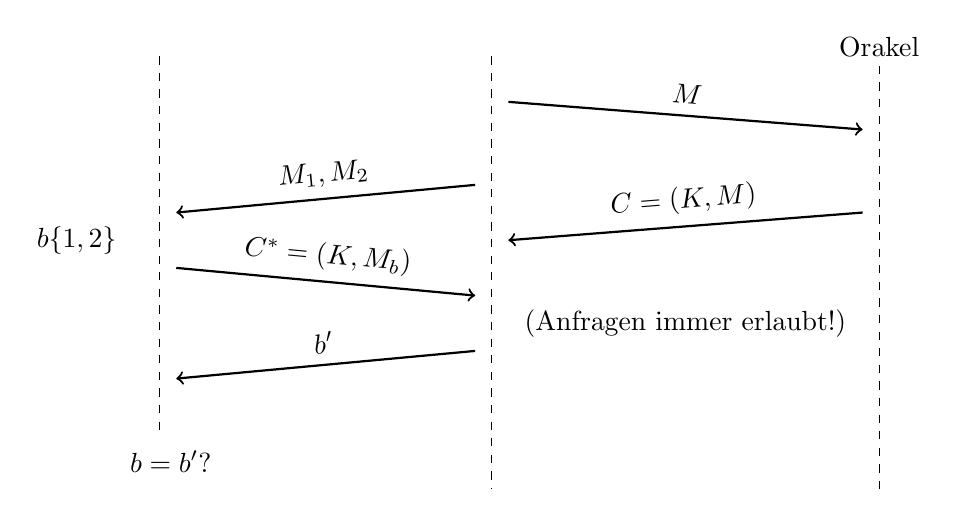
\begin{tikzpicture}[x=2em, y=2em]
	
	\draw (-6,0) node (C) {$\C$};
	\draw (0,0) node (A) {$\A$};
	\draw (7,0) node (Ork) {Orakel};
	
	\draw[dashed] (C) -- (-6,-7);
	\draw[dashed] (A) -- (0,-8);
	\draw[dashed] (Ork) -- (7,-8);
	
	
	\textbf{\draw[->, thick] (0.3,-1) -- (6.7,-1.5) node[sloped,above,pos=0.5] {$M$};}
	
	\textbf{\draw[->, thick] (6.7,-3) -- (0.3,-3.5) node[sloped,above,pos=0.5] {$C = \enc(K, M)$};}
	
	\draw (3.5,-5) node (exp) {(Anfragen immer erlaubt!)};
	
	
	\textbf{\draw[->, thick] (-0.3, -2.5) -- (-5.7,-3) node[sloped,above,pos=0.5] {$M_1, M_2$};}
	
	\draw (-7.5,-3.5) node (b1) {$ b \randUnif \{1,2\}$};
	
	\textbf{\draw[->, thick] (-5.7, -4) -- (-.3,-4.5) node[sloped,above,pos=0.5] {$C^* = \enc(K, M_b)$};}
	
	\textbf{\draw[->, thick] (-0.3, -5.5) -- (-5.7,-6) node[sloped,above,pos=0.5] {$b'$};}
	
	\draw (-5.8,-7.5) node (b2) {$ b = b'$?};
	
	
	\end{tikzpicture}
	%}
	\caption{Nachrichtenaustausch während des IND-CPA-Experiments}
\end{figure}
Wir bemerken, dass der IND-CPA-Sicherheitsbegriff beispielsweise impliziert, dass der Schlüssel $K$ schwer, also nicht in Polynomialzeit, berechenbar ist: Angenommen $\A$ kennt $K$, dann kann der Angreifer $C^{\ast}$ entschlüsseln, mit $\plaint_1$ und $\plaint_2$ vergleichen und bricht somit, da $\Pr \left[ \A \textnormal{ gewinnt} \right] - \frac{1}{2} = 1 - \frac{1}{2}$, die IND-CPA-Sicherheit des zugrundeliegenden Verschlüsselungsverfahrens.

%Semantische Sicherheit heißt Chiffrat darf nicht helfen - aus Chiffraten können keine neuen Informationen effizient berechnet werden, die nicht sschon vorher effizient berechenbar waren
 
\begin{theorem}
Ein Verfahren ist genau dann semantisch sicher, wenn es IND-CPA-sicher ist.
\end{theorem}

Da der Beweis dieser Aussage über das Niveau einer einführenden Kryptographie-Vorlesung hinausgeht, wollen wir an dieser Stelle auf eine Ausführung verzichten und verweisen den interessierten Leser auf die Arbeit von Goldwasser und Micali \cite{Goldwasser1984}. Bemerken möchten wir jedoch, dass die Autoren nicht von der IND-CPA-Sicherheit eines Verschlüsselungsverfahrens sprechen, sondern ein entsprechendes Verfahren als "`polynomial secure"' bezeichnen. 

\subsection{Beispiel ECB-Modus}
\begin{description} 
	\item[Behauptung] Keine Blockchiffre ist im ECB-Modus IND-CPA-sicher.
	\item[Beweis] Betrachte folgenden Angreifer $\A$:
	\begin{itemize}
		\item $\A$ wählt zwei Klartextblöcke $\plaint_1 \neq \plaint_2$ beliebig.
		\item $\A$ erhält  $\ciphert^{*} := \enc(\key, \plaint_{b})$ für zufällig gleichverteilt gewähltes $b \in \{1, 2\}$.
		\item $\A$ erfragt $\ciphert_1 = \enc(\key, \plaint_1)$ durch sein Orakel.
		\item $\A$ gibt 1 aus, genau dann, wenn $\ciphert_1 = \ciphert^{*}$, sonst gibt er 2 aus.
		\item $\Pr \left[ \A \text{ gewinnt} \right] = 1$, also ist das Schema nicht IND-CPA-sicher.
	\end{itemize}
\end{description}
Bei diesem Beispiel nutzt der Angreifer die Schwäche des ECB-Modus, dass gleiche Klartextblöcke immer zu gleichen Chiffrat-Blöcken werden, aus.

\subsection{Beispiel CBC-Modus}
Wie wir bereits im Abschnitt~\ref{ssec:cbc} gelernt haben, gilt bei der Verwendung des CBC-Modus: 
\begin{align*}
\ciphert_i = \enc(\key, \plaint_i \oplus \ciphert_{i-1}) \text{, mit } \ciphert_0 := IV.
\end{align*}
Im Folgenden nehmen wir an, dass der Initialisierungsvektor $IV$ bei jeder Verschlüsselung zufällig gleichverteilt gewählt wird. Somit wird verhindert, dass sich der Modus bei einem einzelnen Datenblock gleich dem ECB-Modus verhält. Im CBC-Modus existiert diese Problematik für längere Nachrichten, selbst bei festem und öffentlichem $IV$, generell nur für den ersten Datenblock, da darauffolgende Datenblöcke mit den vorausgehenden Chiffraten verkettet werden und somit kein direkter Zusammenhang mehr zwischen Daten- und Chiffratblock besteht. Allerdings werden bei der IND-CPA-Sicherheit zwei einzelne Blöcke verwendet, weshalb wir hier auf die Variante mit zufälligem $IV$ ausweichen.

Das zufällige Wählen eines $IV$ löst zwar ein Problem, erzeugt jedoch ein anderes: Um eine korrekte Entschlüsselung zu gewährleisten, muss der gewählte $IV$ mitgesendet werden. Das resultierende Problem ist nun, dass ein Angreifer eben diesen $IV$ verändern kann und somit beliebige Manipulationen am ersten Block einer bekannten Nachricht vornehmen kann.

\begin{description} 
	\item[Behauptung] Eine Blockchiffre ist im CBC-Modus genau dann IND-CPA-sicher, wenn die Verschlüsselungsfunktion $\enc(\key,\cdot): \{0,1\}^l \rightarrow
	\{0,1\}^l$ nicht von einer Zufallsfunktion $R: \{0,1\}^l \rightarrow \{0,1\}^l$ unterscheidbar ist.
	\item[Beweisidee]~
	\begin{description}
		\item[IND-CPA-sicher $\Rightarrow$ Ununterscheidbarkeit]~\\
		$\Leftrightarrow$ IND-CPA-unsicher $\Leftarrow$ Unterscheidbarkeit~\\
		Wenn ein Angreifer $\enc(\key, \cdot)$ von einer Zufallsfolge unterscheiden kann, ist zwischen mindestens zwei Verschlüsselungsergebnissen ein Zusammenhang erkennbar. Es gibt somit mindestens einen Fall, bei dem der Angreifer zusätzliche Informationen für das Zuordnen des Chiffrats besitzt. Daher gilt für zufällig gewählte Nachrichten im IND-CPA-Experiment: Pr$[\A$ gewinnt$] > \frac{1}{2} \Rightarrow$ IND-CPA-unsicher.
		\item[IND-CPA-sicher $\Leftarrow$ Ununterscheidbarkeit]~\\
		Wenn die Verschlüsselungsfunktion aus Sicht des Angreifers nicht von einer Zufallsfunktion unterscheidbar ist, gibt es keine bekannten Zusammenhänge der Verschlüsselungen. Somit ist die Wahrscheinlichkeit, dass der Angreifer ein Chiffrat korrekt zuordnet, genau $\frac{1}{2}$.
	\end{description}
\end{description}

\section{Der IND-CCA-Sicherheitsbegriff}
Der CPA-Angreifer ist mit Zugriff auf ein Verschlüsselungsorakel ausgestattet. Er kann sich jedmöglichen Klartext verschlüsseln lassen und
versuchen, Muster in den Ausgaben des Orakels zu erkennen. Eingeschränkt ist er dennoch, da ihm die Möglichkeit fehlt, zu beliebigen
Ciphertexten den Klartext zu berechnen. Ein stärkerer Sicherheitsbegriff ist daher IND-CCA. Ähnlich wie IND-CPA, steht IND-CCA abkürzend für \emph{indistinguishability under chosen-ciphertext attacks}. Dabei suggeriert das Akronym CCA bereits einen mächtigeren Angreifer. Das in \ref{def:ind-cpa} vorgestellte Experiment können wir problemlos auf einen IND-CCA-Angreifer anpassen. Modifiziert ergibt sich:

\begin{itemize}
	\item Der Angreifer $\A$ besitzt Zugriff auf ein $\enc(\key,\cdot)$-Orakel und ein $\dec(\key,\cdot)$-Orakel
	\item $\A$ wählt zwei Nachrichten $\plaint_1$ und $\plaint_2$ gleicher Länge
	\item $\A$ erhält $\ciphert^{*} := \enc(\key, \plaint_{b})$  für ein zufällig gleichverteilt gewähltes $b \in \{1, 2\}$.
	\item $\A$ gewinnt, wenn er $b$ korrekt errät.
\end{itemize} 

Natürlich darf der Angreifer den Klartext zum Chiffrat $\ciphert^{*}$ nicht bei dem Entschlüsselungsorakel erfragen. Ein Angriff wäre ansonsten trivial und es gäbe kein Verfahren, dass dem IND-CCA-Sicherheitsbegriff genügt. 

%Wieso braucht man hier das hardcoded Leerzeichen und oben nicht?%
Analog heißt ein Verfahren nun IND-CCA-sicher, wenn der Vorteil des Angreifers gegenüber dem Raten einer Lösung, also $\text{Pr} \left[ \A\ \text{gewinnt} \right] - \frac{1}{2}$, für alle Angreifer vernachlässigbar klein ist.

Etwas granularer kann bei IND-CCA zwischen einer adaptiven und einer nichtadaptiven Variante unterschieden werden. Erstere erlaubt dem Angreifer weitere Berechnungen, auch nachdem $\ciphert^{*}$ bereits erhalten wurde, wohingegen die nichtadaptive Variante solche Berechnungen explizit verbietet. In der Theorie kann sich ein adaptiver Angreifer also auch von $\ciphert^{*}$ abhängige Ciphertexte entschlüsseln lassen. Sprechen wir in diesem Skript von IND-CCA, so gehen wir von der adaptiven Variante aus.

%\section{Sicherheitsparameter und effiziente Angreifer}\label{sec:secparam}
%Zu einer Funktion, für die sicherheitsrelevante Eigenschaften gefordert werden, wird in der Kryptographie oft ein \emph{Sicherheitsparameter} $k$ definiert. Informell gesagt, legt $k$ das Sicherheitsniveau der Funktion fest. Beispielsweise parametrisiert er den Bildbereich einer \hyperref[cha:hash]{Hashfunktion}, wo ein größerer Bildbereich bei gleichem Urbildbereich zu einer geringeren Kollisionswahrscheinlichkeit führt.
%\begin{beispiel}
%	Um die Intuition rechnerisch zu belegen, definieren wir eine Funktion
%	\begin{align*}
%		H : \{0, 1\}^{1024} \rArrow \{0, 1\}^{k}\, ,
%	\end{align*}
%	wobei, falls $k = 512$,
%	\begin{align*}
%		\Pr \left[ \exists x' \neq x : H(x') = H(x) \mid x \stackrel{\$}{\longleftarrow} \{0, 1\}^{1024} \right] > \frac{1}{2}
%	\end{align*}
%	und falls $k = 256$,
%	\begin{align*}
%		\Pr \left[ \exists x' \neq x : H(x') = H(x) \mid x \stackrel{\$}{\longleftarrow} \{0, 1\}^{1024} \right] > \frac{3}{4}
%	\end{align*}
%\end{beispiel}
%Ein weiteres Beispiel für die Anwendung des Sicherheitsparameters findet sich bei Verschlüsselungsverfahren, bei welchen die durch $k$ festgelegte Länge des Schlüssels den Aufwand einer Brute-Force-Attacke bestimmt. Dabei wird $k$ vor der Schlüsselerzeugung ausgehandelt und es kann davon ausgegangen werden, dass eine ehrliche Partei sich an die Abmachung hält.
%Die Sicherheit des Verfahrens darf allerdings nicht von der Geheimhaltung des Sicherheitsparameters abhängen. 
%
%Zur Analyse der Sicherheitseigenschaften eines kryptographischen Verfahrens betrachtet man üblicherweise einen Angreifer, der \emph{effizient}, das heißt in seiner Rechenzeit eingeschränkt ist. Intuitiv wird in der Komplexitätstheorie ein effizienter Algorithmus mit einer polynomial-beschränkten Laufzeit in der Eingabegröße gleichgesetzt. 
%In anderen Worten ist ein Algorithmus bei Eingabe eines Bit-Strings der Länge $n$ genau dann effizient, wenn es ein $c \in \mathbbm{N}$ gibt, so dass seine Laufzeit im schlechtesten Fall in $O(n^c)$ liegt.
%Um mit dieser Idee konsistent zu bleiben, wird in der Kryptographie einem Angreifer auf ein Verfahren ein Bit-String $1^k$ von $k$ Einsen übergeben, um die Rechenzeit durch den zugrundeliegenden Sicherheitsparameter zu begrenzen. 
%Ein effizienter Angreifer muss also in $O(k^c)$-Schritten, $c \in \mathbbm{N}$, eine Lösung berechnen. Somit ist beispielsweise die eingangs erwähnte Brute-Force-Attacke auf einen Schlüsselraum $\{0, 1\}^{k}$ ausgeschlossen, da die Laufzeit in $O(2^{k})$ liegt, also exponentiell ist.
%Neben der Begrenzung der Rechenzeit erlauben wir einem Angreifer, um ein realistisches Szenario abzubilden, zu jedem Zeitpunkt eine \emph{faire} Münze zu werfen, das heißt, eine Lösung zu raten. Einen solchen Angreifer bezeichnen wir als \emph{probabilistic polynomial time} (PPT) Angreifer.
%%Was ist mit den Längen der anderen Eingaben, die ein Angreifer bekommt?
%
%Damit ein Verschlüsselungsverfahren grundsätzlich als sicher angenommen werden kann, muss die Erfolgswahrscheinlichkeit eines Angreifers möglichst klein sein und darf idealerweise nur vom Zufall abhängen.
%Da der Sicherheitsparameter für jedes Verfahren beliebig variiert werden kann, erscheint es intuitiv logisch, die Sicherheit nicht in Abhängigkeit der Größe von $k$ zu definieren. Vielmehr fordern wir für eine bestimmte Sicherheitseigenschaft, dass ein PPT Angreifer die Charakteristik nur mit \emph{vernachlässigbarer} Wahrscheinlichkeit in $k$ brechen kann.
%\begin{definition}[Vernachlässigbarkeit]
%	Es sei $f$ eine Funktion, $k$ eine Konstante und $p(\cdot)$ ein beliebiges Polynom. Dann heißt $f$ vernachlässigbar in $k$, wenn
%	\begin{align*}
%		\exists k_0 : \forall k \geq k_0 : \vert f(k) \vert \leq \frac{1}{p(k)} 
%	\end{align*}
%\end{definition}
%Beispielsweise ist $f = \frac{1}{2^k}$ vernachlässigbar in $k$, $f = \frac{1}{k^2}$ jedoch nicht.
%
%Dass ein Verfahren in der Praxis bei zu klein gewähltem Sicherheitsparameter, trotz vernachlässigbarer Erfolgswahrscheinlichkeit eines PPT Angreifers, keine Sicherheit bieten kann, ist trivial.